\section{Client}
Il programma client tenta di stabilire immediatamente una connessione TCP con il server: in caso di esito positivo, dà la possibilità all'utente di interagire con il sistema attraverso una riga di comando, e interrompe con esito negativo l'esecuzione in caso contrario.

A differenza del server, il client non si serve di alcuna persistenza dei dati, ma necessita in ogni caso di una directory di lavoro da sfruttare per la memorizzazione dei file che gli vengono inviati dal server per permettere la modifica delle sezioni o per la ricezione del contenuto attuale dei documenti. Il meccanismo utilizzato per la verifica dell'esistenza e validità di tale directory è identico a quello utilizzato dal server.

\paragraph{Thread Life-cycle}
Lo scambio di comandi e risultati avviene all'interno del thread principale, ma viene delegata a thread secondari la gestione delle notifiche e la ricezione dei messaggi multicast diretti al gruppo di cui il client è membro.

\begin{figure}[h]
	\caption{Client - Ciclo di vita dei Thread}
	\centering
	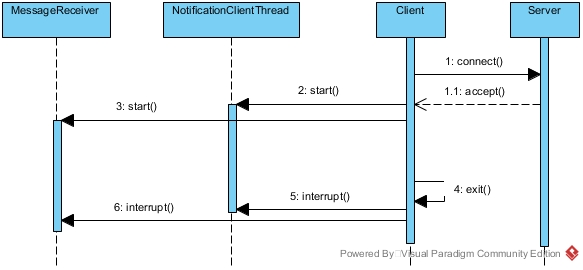
\includegraphics[scale=0.5]{assets/client/thread_activation_sequence_diagram}
\end{figure}